\section{Results}
\label{sec:results}

\para{Bereavement does not widen the authenticity gap.}
\begin{table}[t]
    \centering
    \resizebox{\textwidth}{!}{%
    \begin{tabular}{@{}lccccc@{}}
        \toprule
        Domain & Human Auth. & Model Auth. & Diff. & 95\% CI & Welch $p$ \\
        \midrule
        Bereavement & {\bf 4.92} & 4.75 & 0.17 & [$-0.08$, 0.42] & 0.213 \\
        Other grief & {\bf 4.67} & 4.54 & 0.13 & [$-0.08$, 0.38] & 0.355 \\
        \bottomrule
    \end{tabular}%
    }
    \caption{Authenticity by domain and source. Human passages score slightly higher in both domains, but the gaps are small and statistically inconclusive. Best values within each row are in \textbf{bold}.}
    \label{tab:authenticity-main}
\end{table}

As shown in \tabref{tab:authenticity-main}, human passages score slightly higher than model passages in both domains, but the absolute gaps are small: 0.17 points in bereavement and 0.13 points in other grief. Neither contrast is statistically significant under Welch's $t$-test, and both remain non-significant after FDR correction. \Figref{fig:authenticity-by-domain} visualizes the same pattern. The key interaction test is also null: the source-by-other-grief coefficient is $+0.042$ with $p=0.835$ and $R^2=0.197$. In other words, bereavement does not enlarge the human-model authenticity gap in this pilot.

\begin{figure}[t]
    \centering
    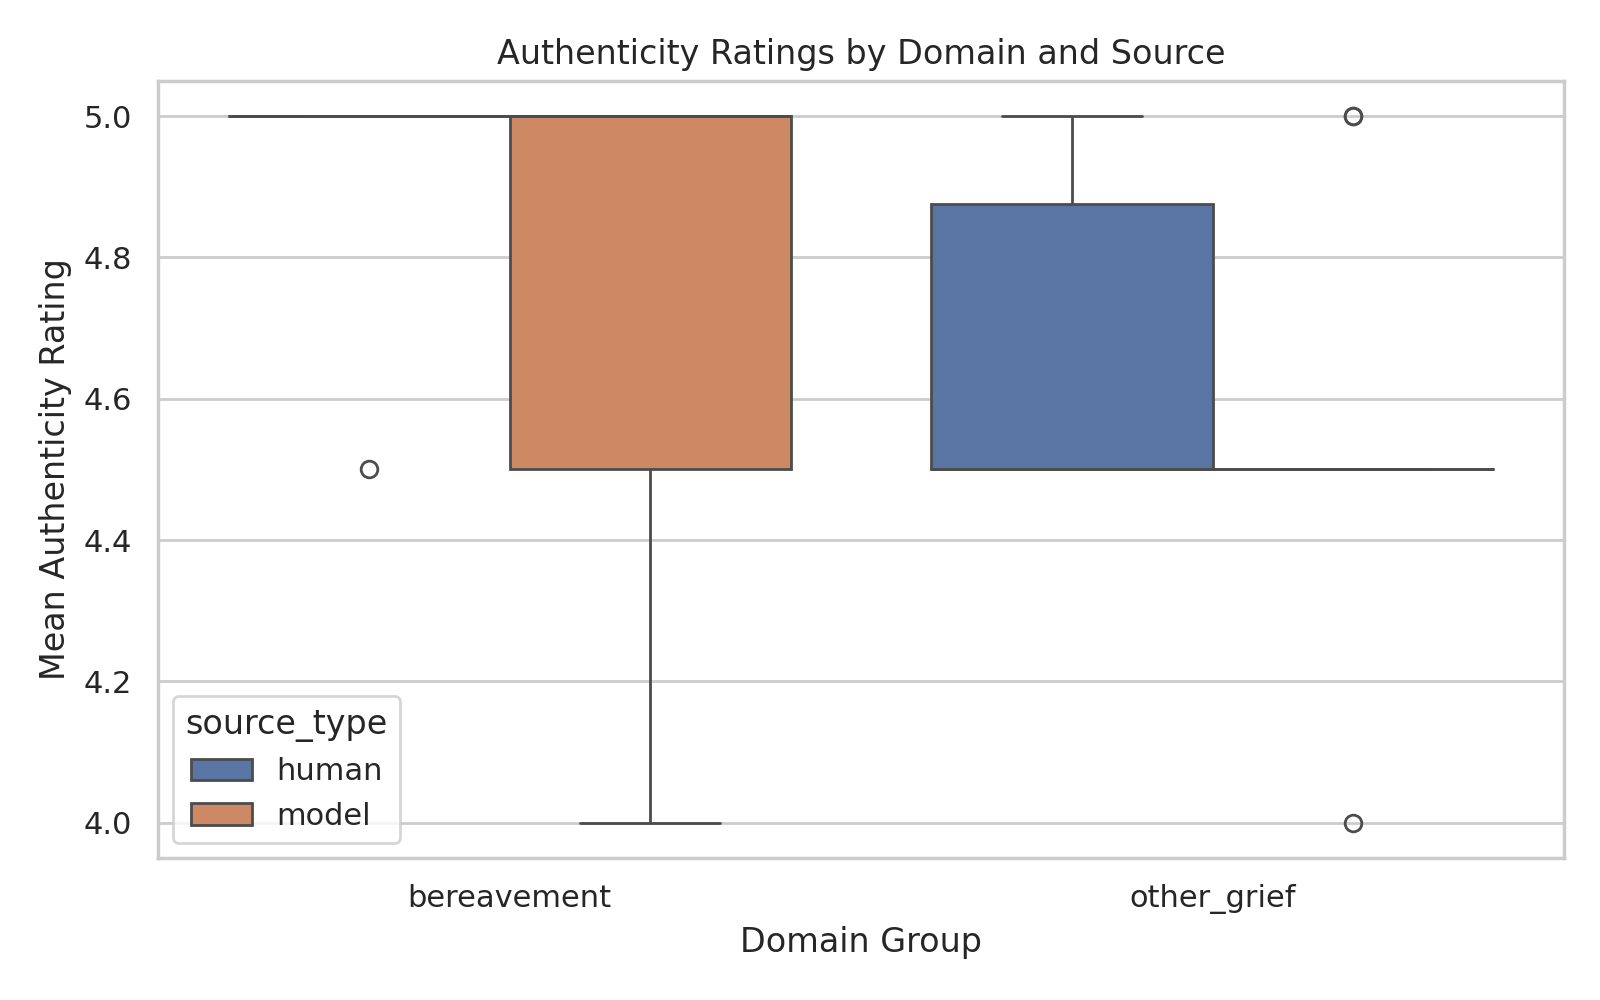
\includegraphics[width=0.95\linewidth]{figures/authenticity_by_domain_source.png}
    \caption{Authenticity scores by domain and source. Human passages score slightly higher on average, but the gap is small in both bereavement and other grief, and the difference does not widen for death-related writing.}
    \label{fig:authenticity-by-domain}
\end{figure}

\para{Judge ratings saturate near the top of the scale.}
Across providers, the mean authenticity score is 4.792 for human texts, 4.708 for \gptfive, and 4.583 for \claudesonnet. Emotional plausibility is similarly high: 4.917 for human texts and 4.750 for both model providers. Specificity also remains high, with \gptfive averaging 5.000. The most striking judge result is categorical: all 72 source guesses label the text as human or human-written. Under this rubric, the judges do not operationally separate sources at all. This ceiling effect is itself informative, because it shows that machine-detection cues were not strong enough to force source discrimination under blinded reading.

\para{Detector separability remains substantial.}
\Figref{fig:detector-authenticity} shows the relationship between detector score and judged authenticity. The \mage detector reaches AUROC $=0.826$ and threshold-0.5 accuracy $=0.750$. At that threshold, 23 of 24 model texts are flagged as machine, but 8 of 12 human texts are also flagged as machine. Mean machine probabilities are 0.998 for bereavement model texts and 0.922 for other-grief model texts, versus 0.665 and 0.596 for the corresponding human groups. The detector therefore retains real source information, but it overcalls ``machine'' on human grief writing in this domain-shifted setting.

\begin{figure}[t]
    \centering
    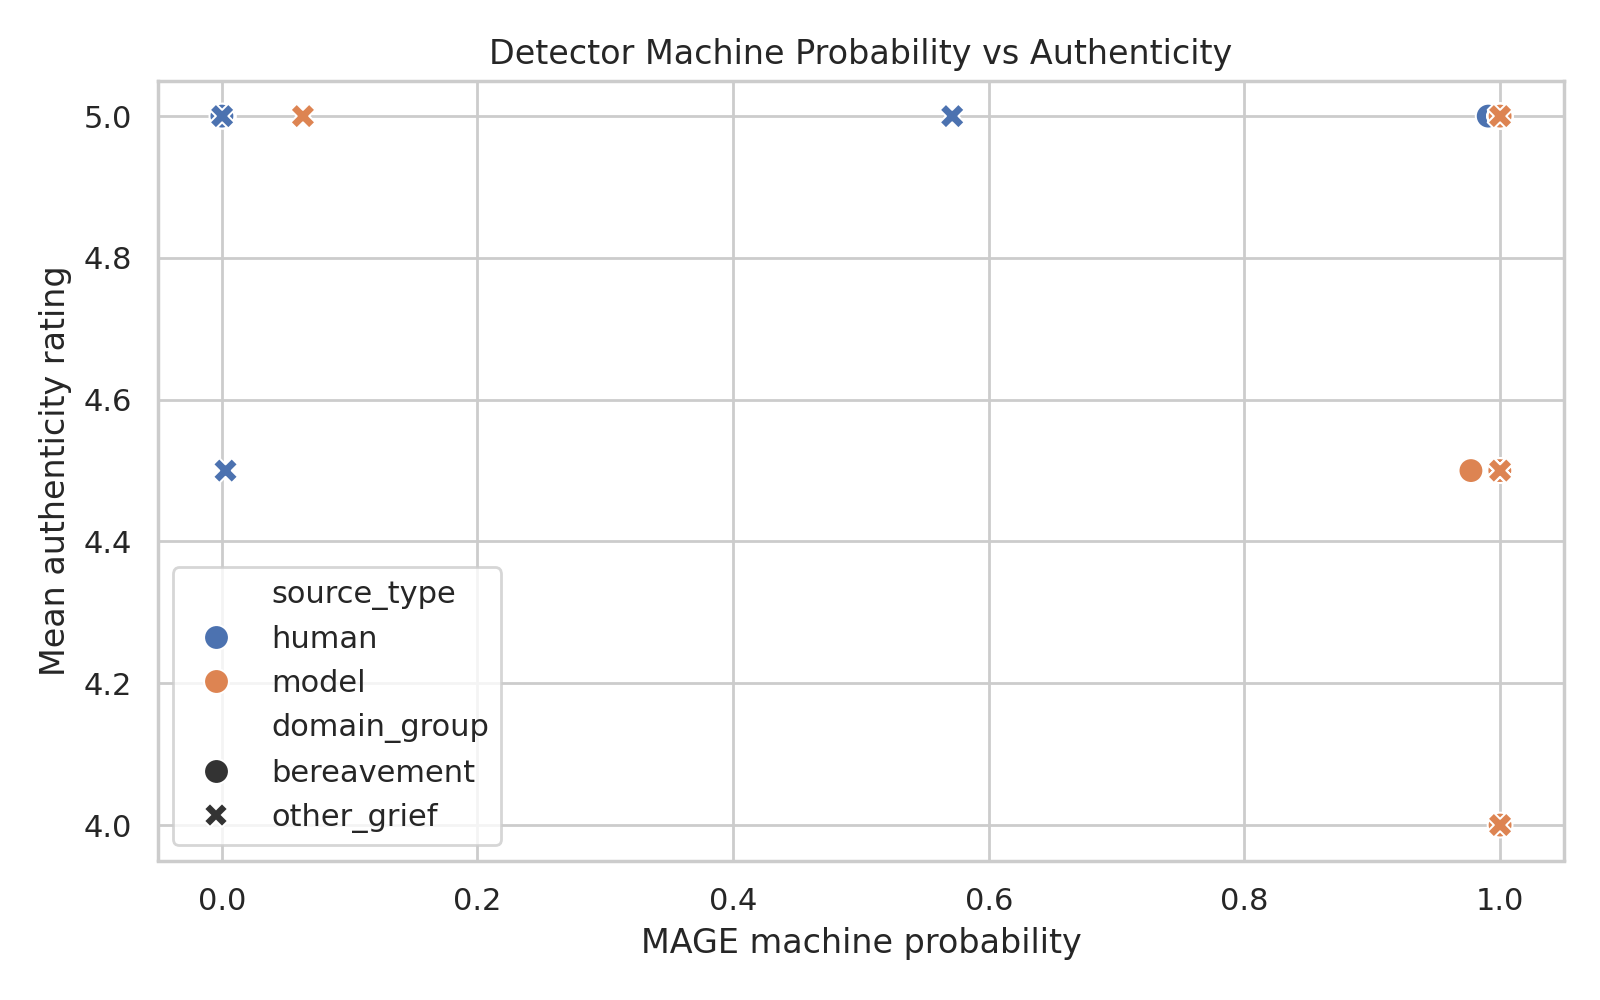
\includegraphics[width=0.95\linewidth]{figures/detector_vs_authenticity.png}
    \caption{Detector machine probability versus judged authenticity. The relationship is weakly negative rather than strongly monotonic, illustrating that texts can appear authentic to blinded judges while still carrying machine-like distributional traces.}
    \label{fig:detector-authenticity}
\end{figure}

The detector-authenticity relationship is weak. Spearman correlation between machine probability and authenticity is $\rho=-0.249$ with $p=0.144$. This is consistent with some overlap between machine-likeness and lower authenticity, but not with a reliable one-to-one mapping.

\para{Model outputs are mildly regularized rather than obviously broken.}
\begin{table}[t]
    \centering
    \resizebox{\textwidth}{!}{%
    \begin{tabular}{@{}lcccccc@{}}
        \toprule
        Provider & Auth. & Plaus. & Specificity & Words & TTR & Object rate \\
        \midrule
        Human & {\bf 4.792} & {\bf 4.917} & 4.875 & 93.1 & 0.686 & {\bf 0.051} \\
        \gptfive & 4.708 & 4.750 & {\bf 5.000} & 102.2 & 0.774 & 0.045 \\
        \claudesonnet & 4.583 & 4.750 & 4.875 & {\bf 108.4} & {\bf 0.782} & 0.041 \\
        \bottomrule
    \end{tabular}%
    }
    \caption{Provider-level means across the blinded text pool. Generated texts are slightly longer and more lexically varied, while human texts retain the highest authenticity, plausibility, and object-word density. Best values in each column are in \textbf{bold}.}
    \label{tab:provider-style}
\end{table}

\tabref{tab:provider-style} summarizes provider-level style features. Model outputs are somewhat longer than human passages and show higher type-token ratios, while object-word rate is slightly lower. \gptfive comes closer to the human authenticity mean than \claudesonnet, but both model families remain high-scoring overall. \Figref{fig:style-features} shows the same descriptive trend graphically. The picture is not one of authenticity collapse. It is closer to stylistic smoothing: model texts look a bit more regularized while still satisfying the judges' criteria for plausible, concrete grief writing.

\begin{figure}[t]
    \centering
    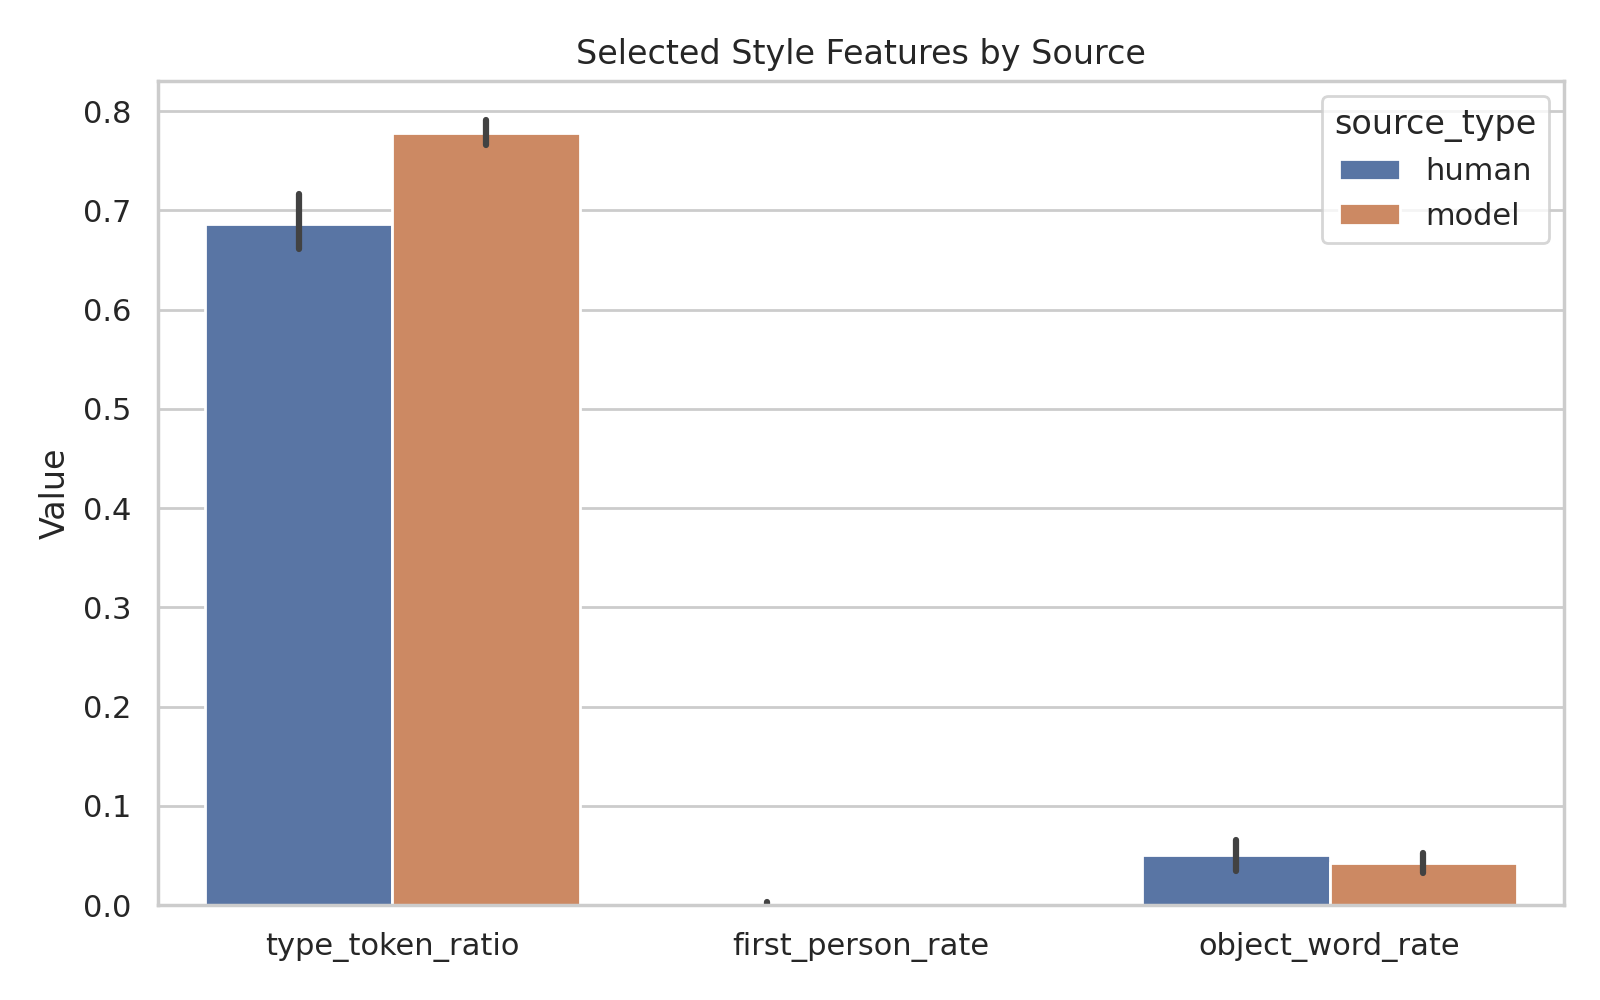
\includegraphics[width=0.95\linewidth]{figures/style_features_by_source.png}
    \caption{Selected style features by source. Generated texts are slightly longer and more lexically varied, with somewhat lower object-word density. These shifts suggest mild stylistic smoothing rather than a sharp failure to produce grief-like prose.}
    \label{fig:style-features}
\end{figure}
